%% The following is a directive for TeXShop to indicate the main file
%%!TEX root = diss.tex

\chapter{Abstract}

% This document provides brief instructions for using the \class{ubcdiss}
% class to write a \acs{UBC}-conformant dissertation in \LaTeX.  This
% document is itself written using the \class{ubcdiss} class and is
% intended to serve as an example of writing a dissertation in \LaTeX.
% This document has embedded \acp{URL} and is intended to be viewed
% using a computer-based \ac{PDF} reader.

% Note: Abstracts should generally try to avoid using acronyms.

% Note: at \ac{UBC}, both the \ac{GPS} Ph.D. defence programme and the
% Library's online submission system restricts abstracts to 350
% words.

% \ifgpscopy
%   This document was typeset in \texttt{gpscopy} mode.
% \else
%   This document was typeset in non-\texttt{gpscopy} mode.
% \fi

% Consider placing version information if you circulate multiple drafts
%\vfill
%\begin{center}
%\begin{sf}
%\fbox{Revision: \today}
%\end{sf}
%\end{center}
\par Graph structured data is used in a variety of applications because it naturally models ubiquitous concepts such as social networks, protein structures, and supply chains \cite{heidari2018scalable, yan2011applications}. This has motivated the development of \acp{GPS} whose aim is to process analytic queries such as PageRank, Shortest Paths, or Connected Components. Previous work accelerated graph processing by modifying the graph's data layout in memory \cite{rabbit, dbg, cost} or on disk \cite{mosaic, basc}. Since we typically describe a graph $G$ in terms of its Vertex and Edge sets using the notation $G(V, E)$, most \acp{GPS} can be categorized as \ac{VC} \cite{graphchi,flashgraph, basc} or \ac{EC} \cite{xstream} dependant on whether the systems implement analytical queries by applying a function over each vertex or each edge. 

\par In the \ac{VC} model, algorithms rely on user-defined vertex programs to compute analytic properties of an input graph. Vertex programs are run iteratively on every vertex in the graph. In each iteration, each vertex executes a user-defined vertex program, and messages are exchanged between neighbouring vertices to propagate updated vertex values. \ac{VC} systems reorder the \textit{vertices} of the graph to improve the locality of vertices that are expected to be frequently accessed together. 

\par In the \ac{EC} model, iteration occurs over the edges of the graph. For each edge in the graph, we apply an update to either the source or destination vertex incident on that edge. \ac{EC} systems reorder the \textit{edges} of the graph to mitigate the random-access pattern of incident vertices that is common to many graph processing kernels such as PageRank.

\par One way of representing a graph is as a square $N \times N$ matrix, $A$, where $N= |V|$. A non-zero element $A_{i, j}$ indicates the existence of an edge from vertex $i$ to vertex $j$. Real-world graphs are typically sparse \cite{listingkcliques}, meaning that the number of edges, $M=|E|$, is much smaller than the number of possible edges in the graph: $M\ll M_{\max} = {N \choose 2}$. 

\par \ac{EC} systems that order the edges of the graph by ascending \textit{Source} or \textit{Destination} ID effectively iterate over $A$ in Row-major or Column-major order, respectively. If we traverse the adjacency matrix of a graph in Row-major order, we will have excellent locality in the source vertices (since we will process all outgoing neighbours of a source vertex before moving on to the next source vertex), but our access to the destination vertex of each outgoing edge will corrsepond to near-random memory accesses of the vertex array. Prior work \cite{cost} addressed this concern by using an edge ordering defined by the \ac{HSFC}, which is a way of assigning indices to the edges of a graph that produces locality in \textit{both} the source and destination vertices. 

\par \ac{VC} systems can use vertex reordering as a preprocessing optimization to improve the memory access locality of the vertices. For example, certain \ac{VC} systems \cite{dbg, cagra} use the degrees of the vertices of the graph to cluster and/or sort the vertices (e.g., sorting the vertices by descending order of degree). The rationale for this optimization is that high degree vertices (also known as ``Hub'' vertices) are, by definition, neighbours of a large number of vertices. These hubs will be frequently accessed when iterating over the edge set of the graph \cite{lwr}. A descending degree sort colocates these hub vertices in memory and increases the likelihood of frequently accessed vertices being cached. Alternatively, Rabbit Order \cite{rabbit} relies on the observation that many real-world graphs such as social networks contain community structures, where vertices that belong to the same community share a larger number of edges than vertices that belong to separate communities. The goal of Rabbit Order is to order the vertices in such a way that consecutive vertex IDs correspond to meaningful communities. The algorithm first detects these communities and then labels the vertices according to those communities. 

\par A vertex reordering can be defined as a function that maps each vertex ID to a new ID in the range: $[0, N)$. This mapping or relabeling is known as a \textit{graph isomorphism}, since all edges between vertices are preserved and the structure of the graph is unchanged. However, observe that vertex reordering can impose ``structure'' on the adjacency matrix of the graph. Figure \ref{fig:fb_adjmats} shows the adjacency matrix of a Facebook social network graph that was constructed from the data of survey participants using the Facebook App \cite{leskovec2012learning}. The graph has been reordered using 3 vertex orders: a random vertex ID assignment, and the IDs calculated using Rabbit and Cuthill-McKee orders. 

\begin{figure*}[!htp]

  \centering
  \subfloat[Random Order]{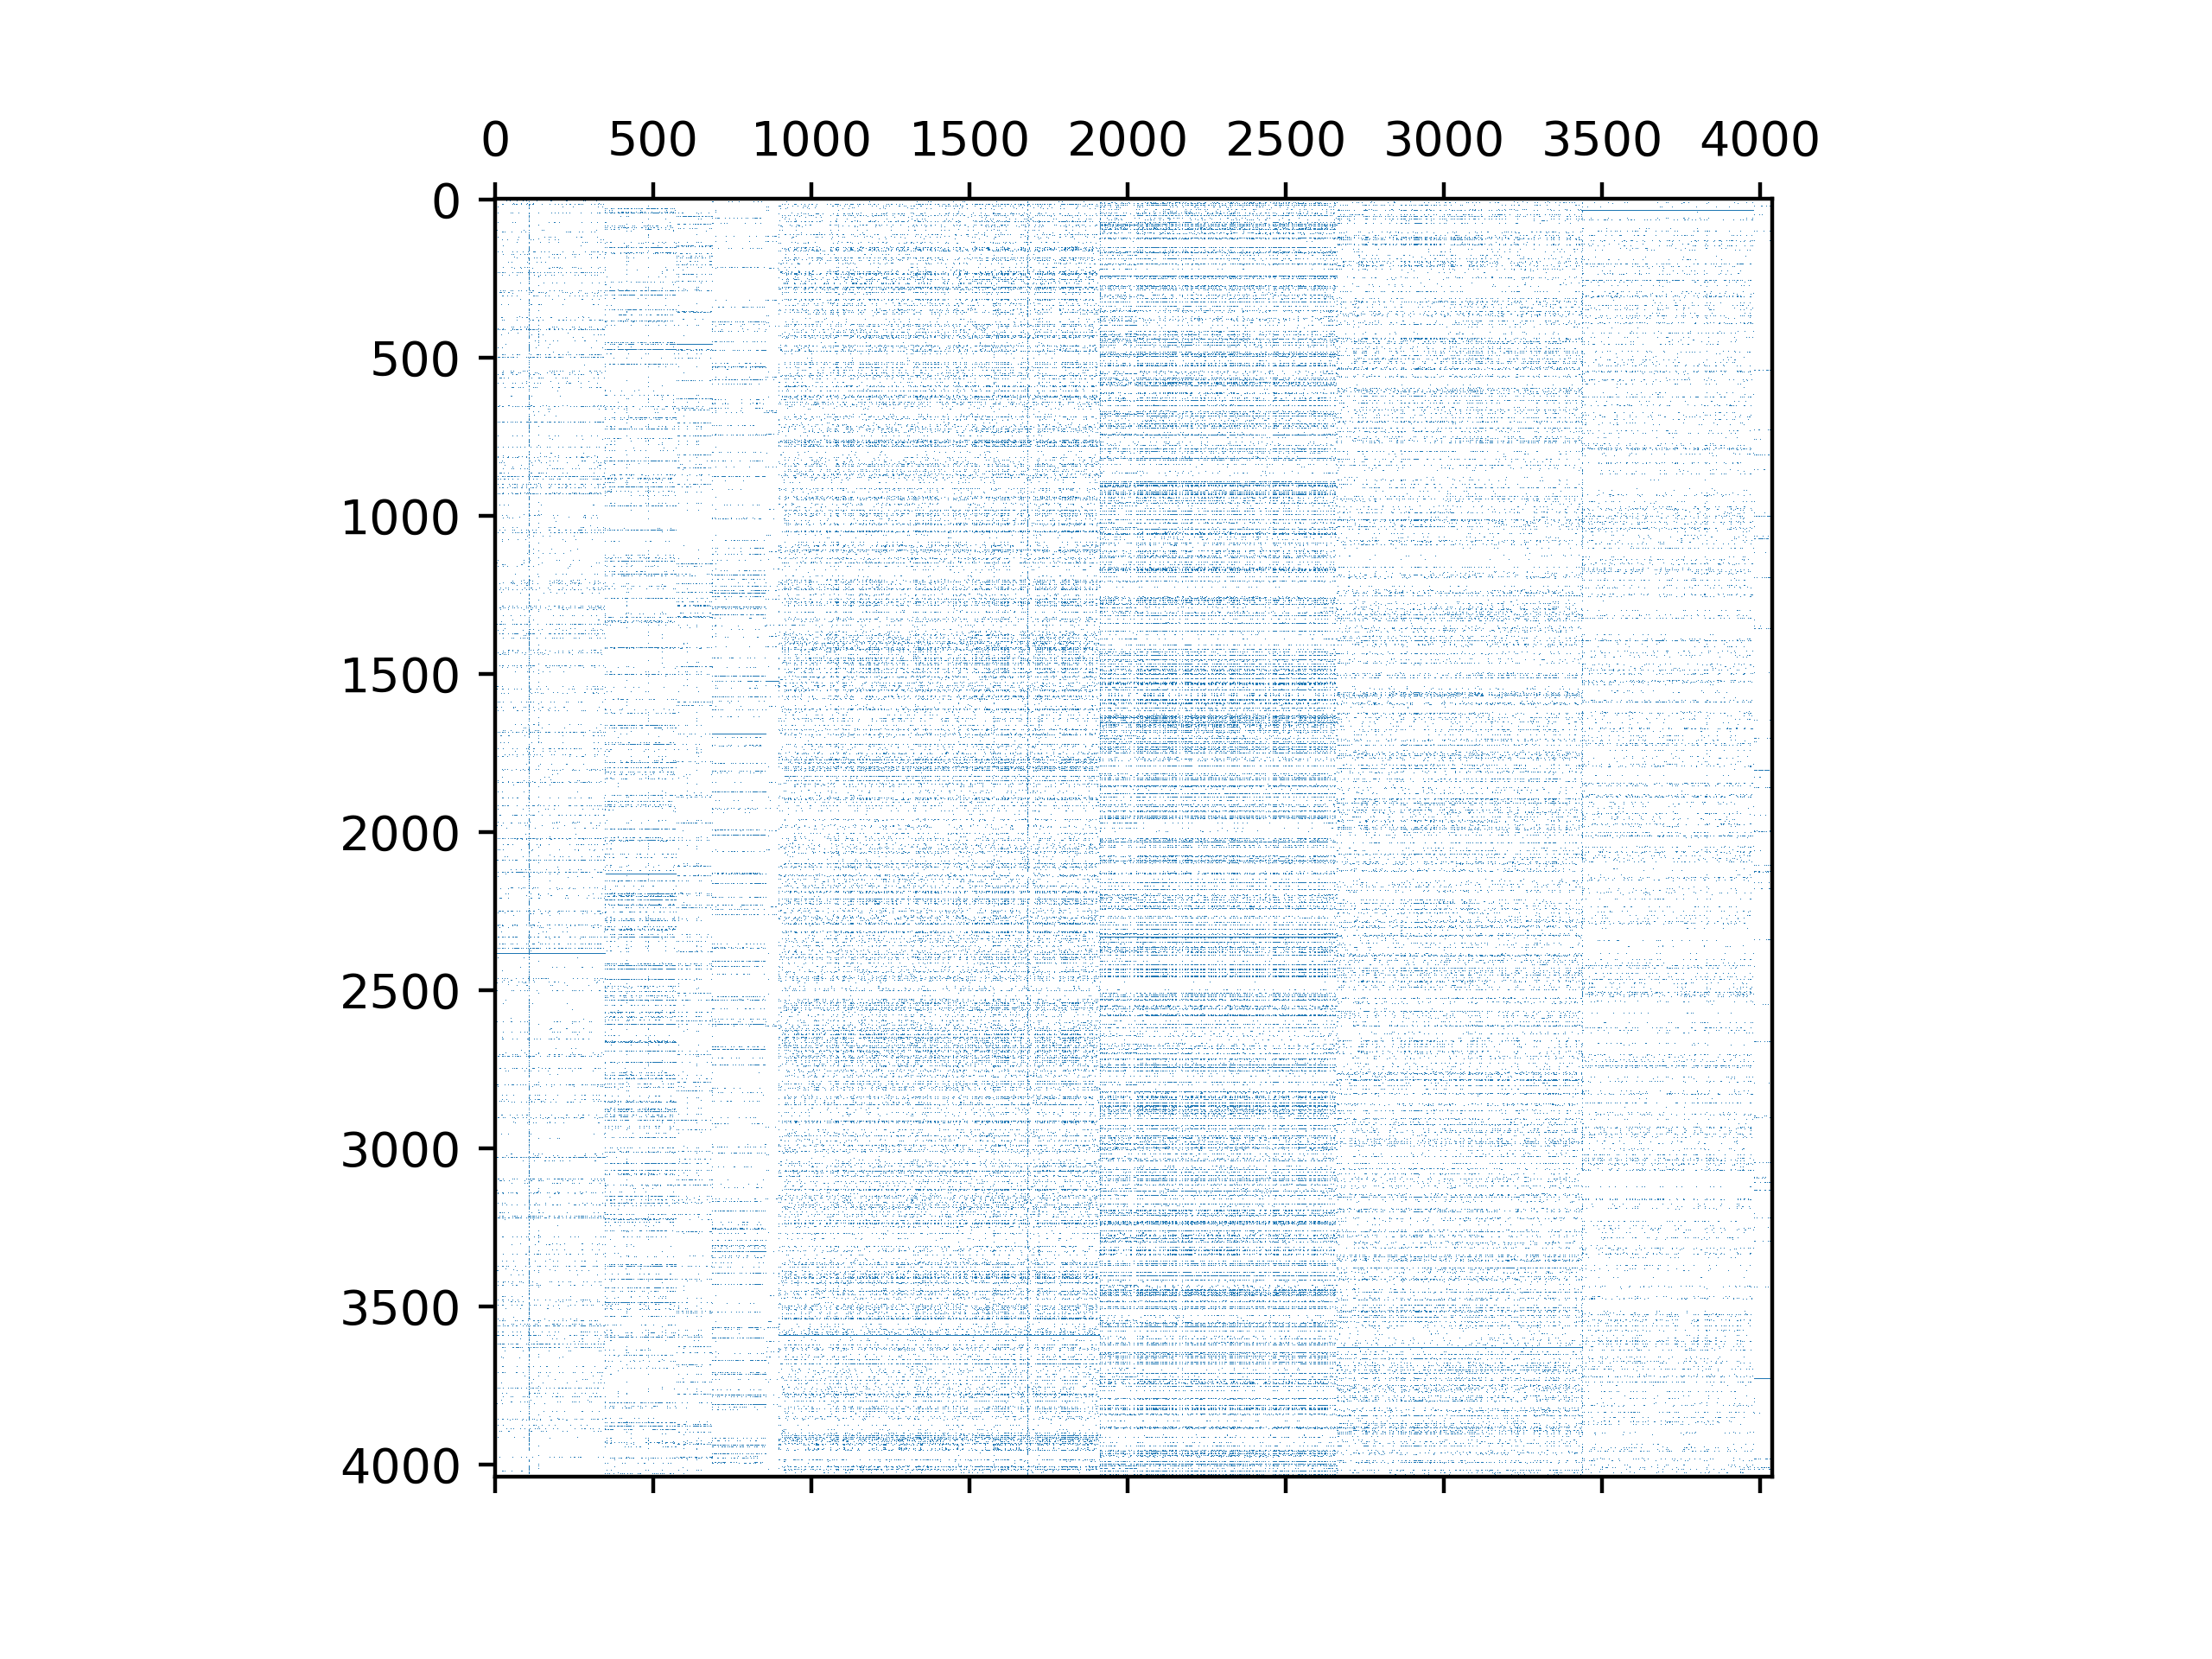
\includegraphics[width=5.5cm]{figures/fb-combined-rnd.png}}\hfil   
  \subfloat[Rabbit Order]{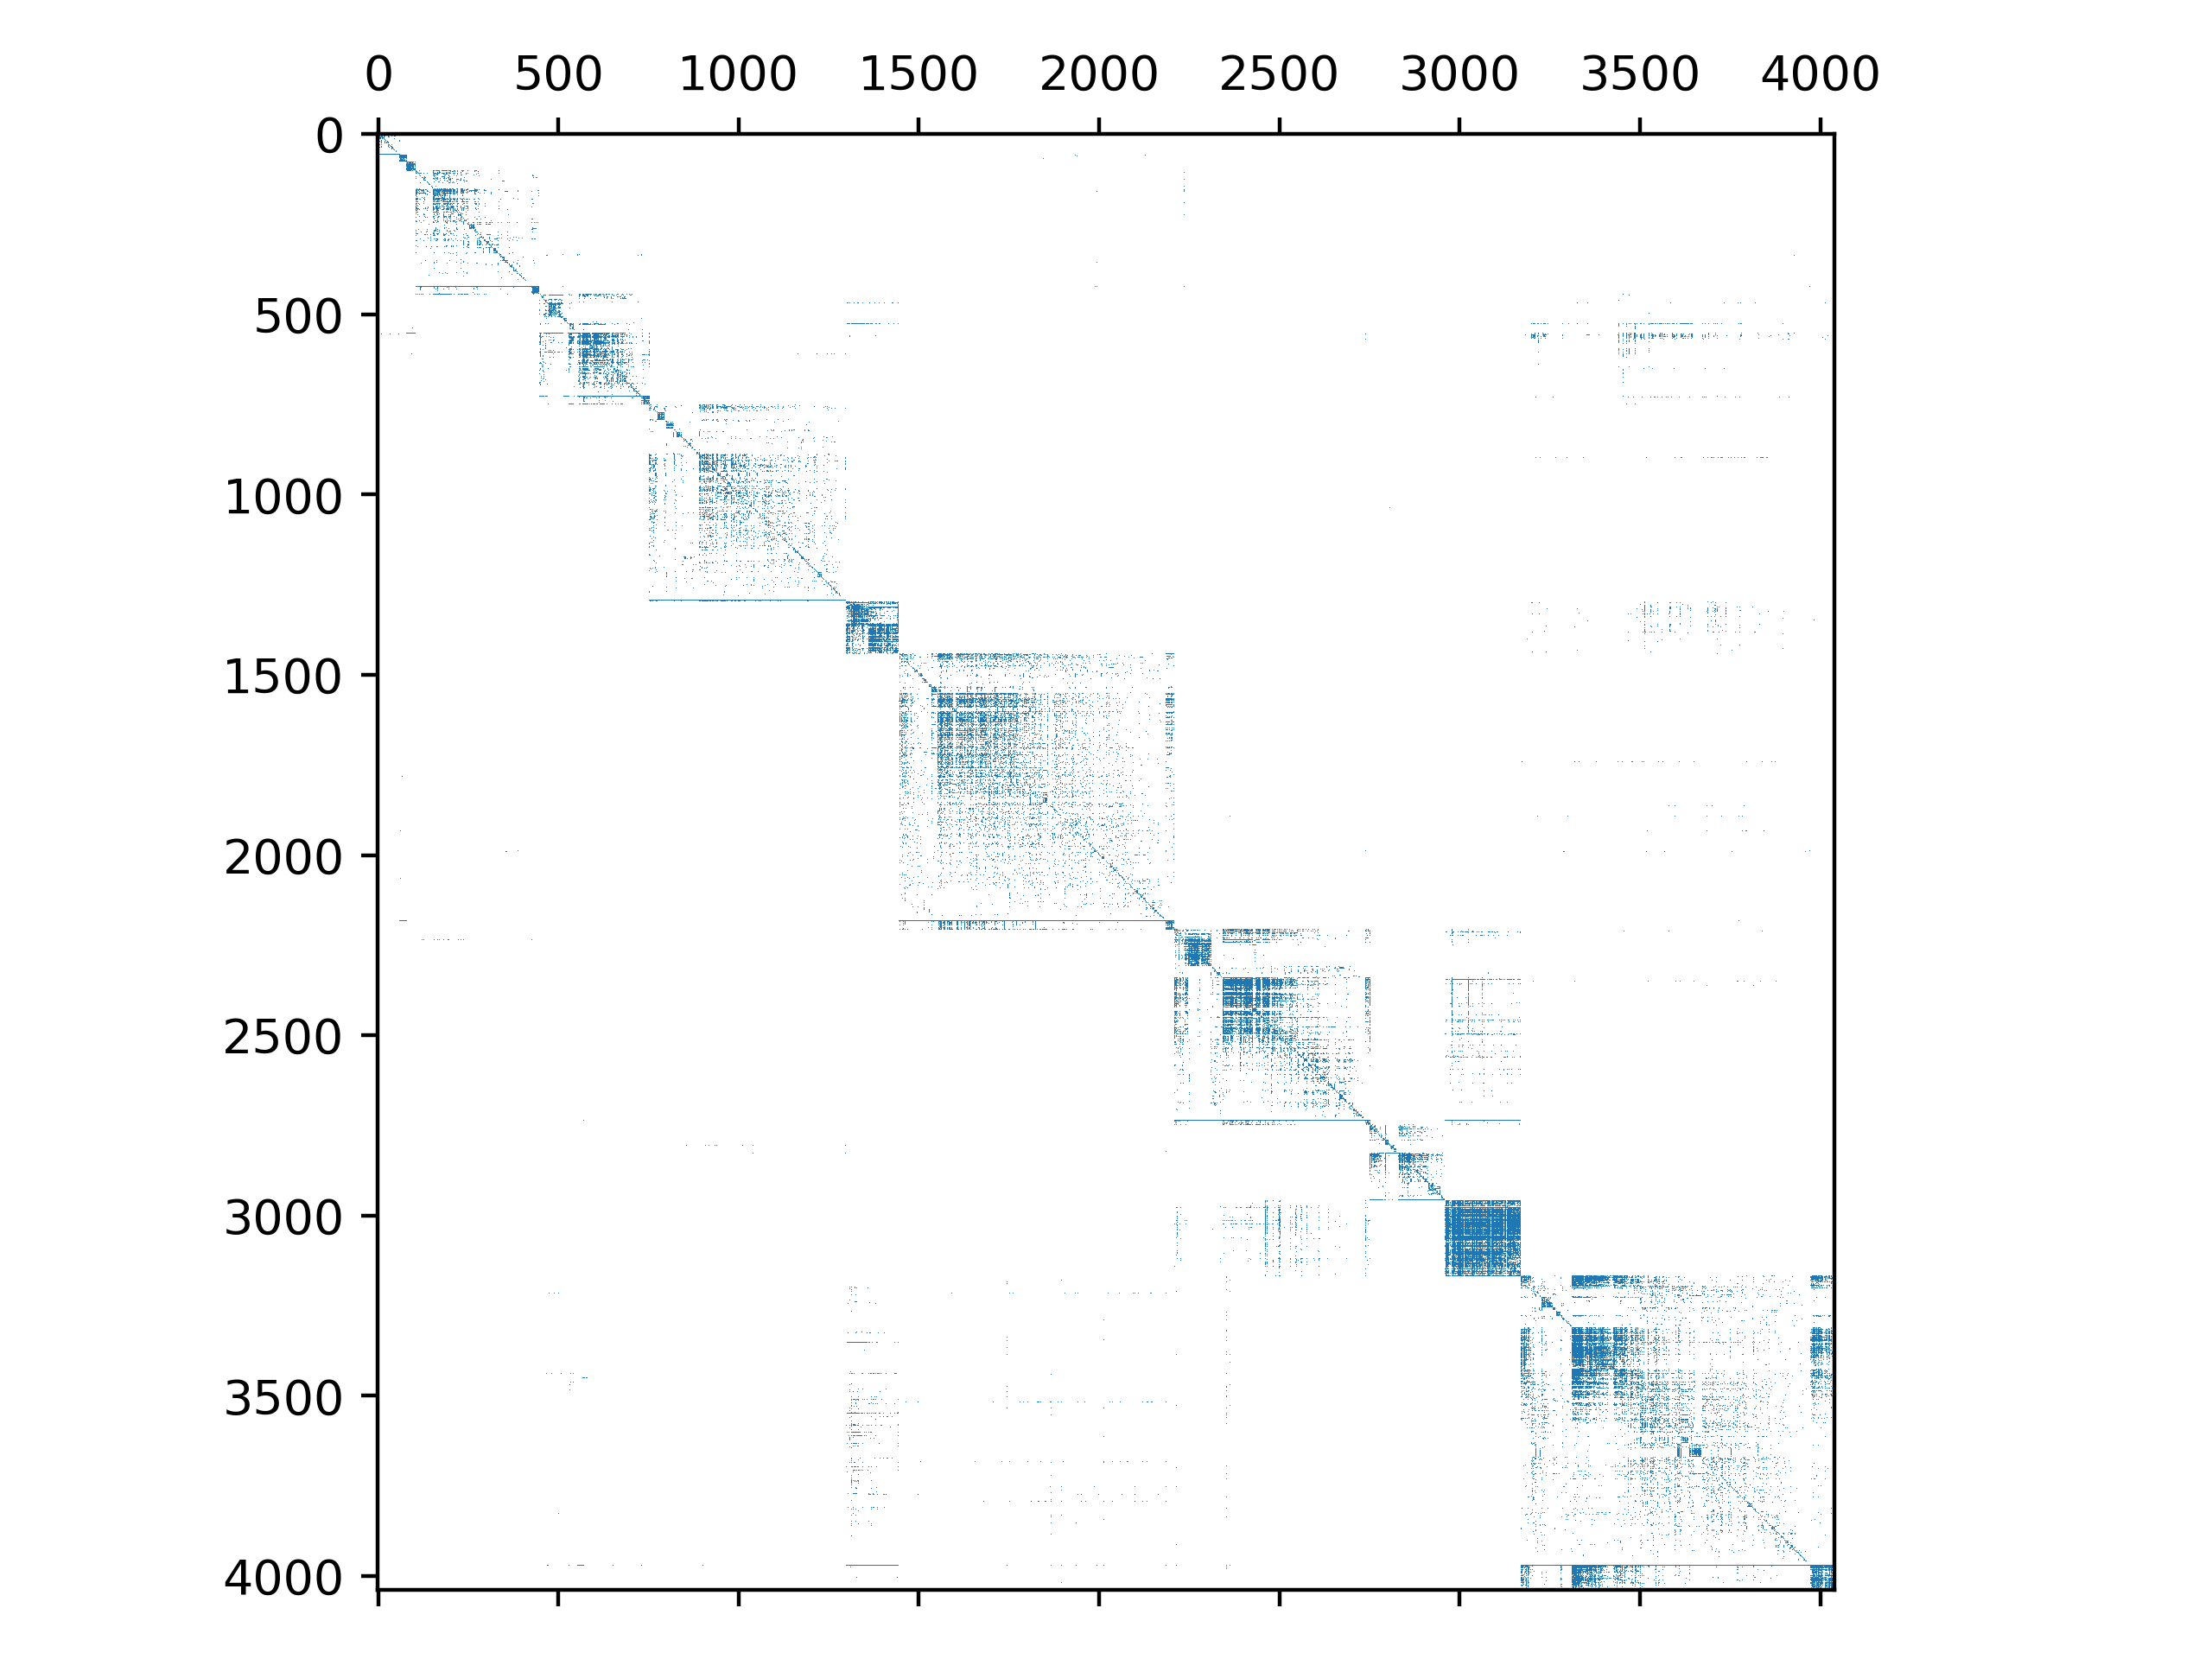
\includegraphics[width=5.5cm]{figures/fb-combined-rbt.png}}\hfil
  \subfloat[Cuthill-McKee Order]{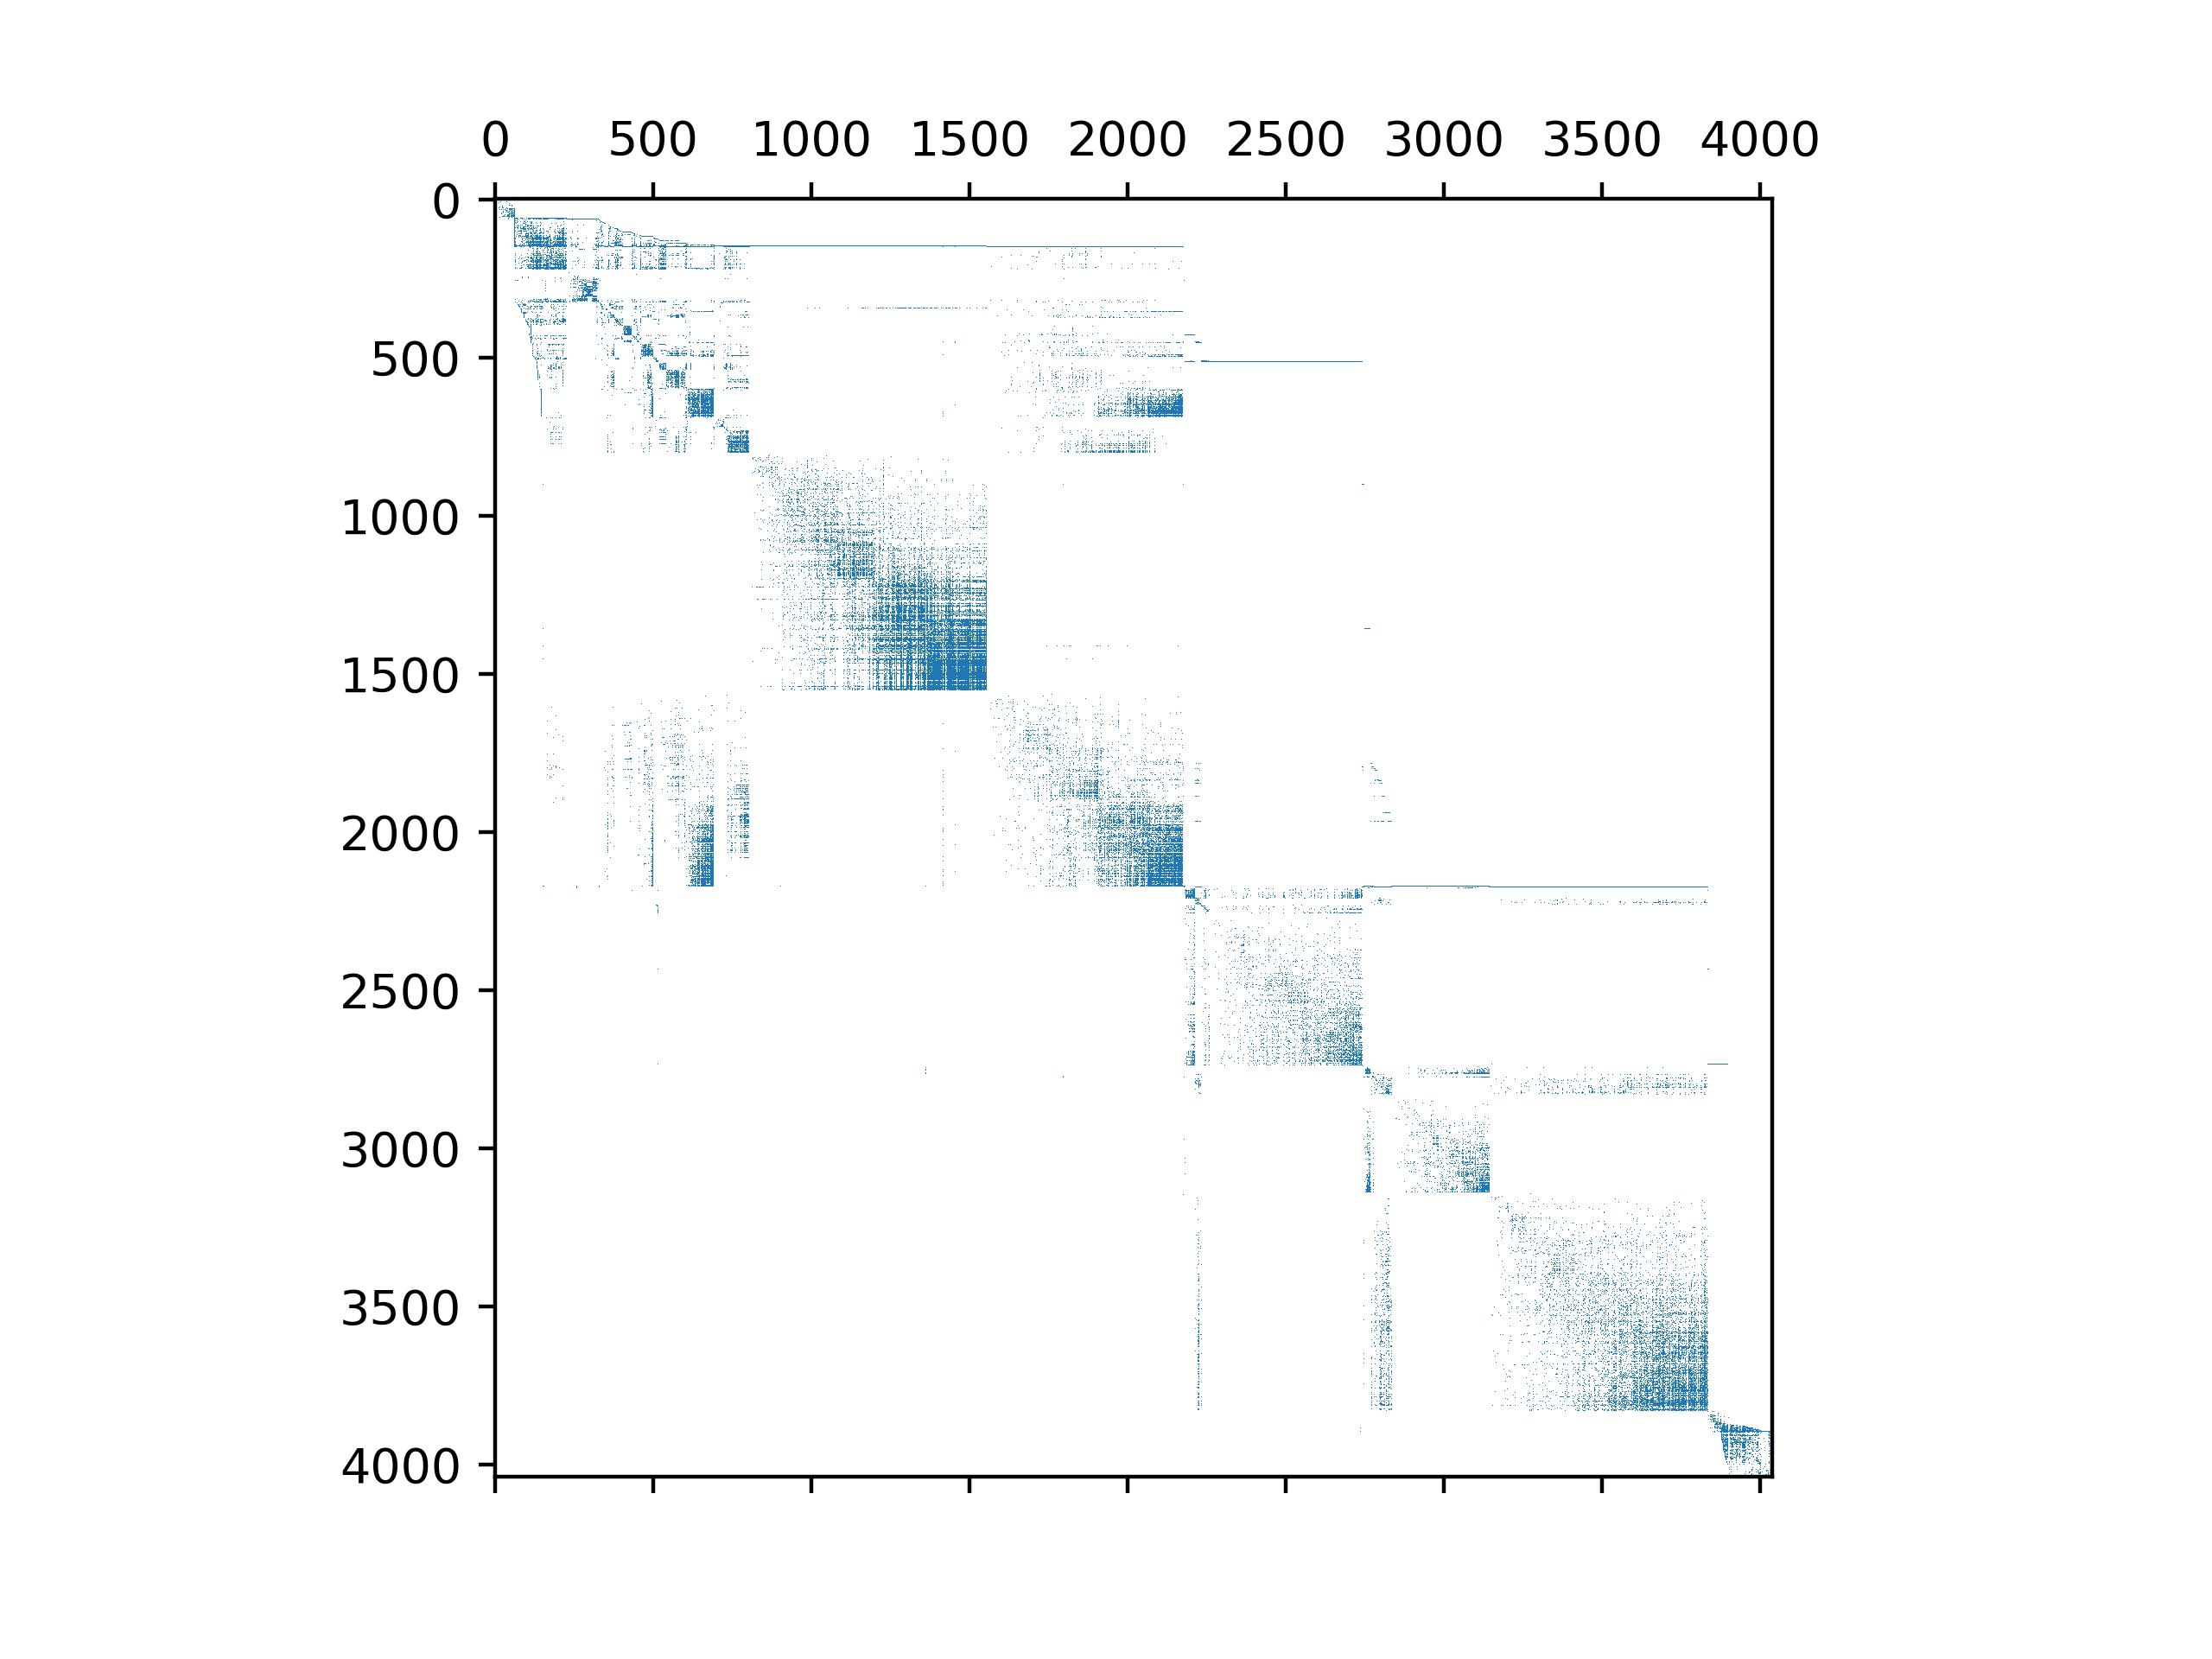
\includegraphics[width=5.5cm]{figures/fb-combined-rcm.png}}
  \caption{Adjacency matrices of an undirected Facebook Social Network graph with 4,039 vertices and 88,234 edges. Each pixel denotes an undirected edge (``friend-of'' relationship) between a pair of vertices (users) in the graph. Note the detected dense communities (submatrices) along the diagonal in (b) and the reduced bandwidth of the sparse matrix in (c). }\label{fig:fb_adjmats}
  \end{figure*}

This thesis is concerned in the interaction between Vertex and Edge ordering. Namely:

\textbf{RQ1}: It has been shown that using vertex and edge ordering to preprocess a graph confers performance benefits in a variety of applications. Is it possible to combine vertex
and edge ordering as a preprocessing step such that the performance benefit gained by the combination of both is compounded (i.e., is greater than using either separately)?
\begin{itemize}
  \item Can edge-centric graph traversal be sped up by first introducing some structure into the adjacency matrix?
\end{itemize}

\textbf{RQ2}: Given an arbitrary input graph, is there a \textit{vertex-and-edge} ordering combination that yields the best performance for an \ac{EC} traversal (measured in speed of execution and number of cache misses)?

This work answers these questions by making the following contributions. We:

\begin{enumerate}
  \item {Perform a preliminary performance evaluation on different vertex and edge orderings on single-threaded \ac{EC} traversals for a variety of graph datasets. We conclude that there \textit{does not} exist a one-size-fits-all \textit{vertex-and-edge} ordering that outperforms all others for all types of graphs.}
  \item {Derive an analytic model of performance using a dataset of graph features (statistical measures that summarize a graph), to identify the characteristics of a graph that help us determine which vertex-and-edge ordering performs best for \ac{EC} workloads.}
  \item {Develop a fully parallel implementation of the SlashBurn vertex ordering technique: \textbf{ParSB}.}
  \item {Propose a novel, lock-free, multithreaded vertex-and-edge ordering technique that leverages the compressed graph representation given by ParSB and traverses the edges of the graph using the \ac{HSFC}.}
  \item {Evaluate our novel vertex-and-edge ordering and compare its performance against locking-based and merging-based multithreaded \ac{EC} traversals.}
\end{enumerate}